\documentclass[a4paper,10pt,twocolumn]{ltjarticle}
\usepackage{kaitoushu}

% グラフ用の共通スタイル定義
\pgfplotsset{
  myaxis/.style={
    axis lines=middle,
    xlabel={$x$}, ylabel={$y$},
    every axis x label/.style={at={(ticklabel* cs:1)},anchor=west},
    every axis y label/.style={at={(ticklabel* cs:1)},anchor=south},
    tick label style={font=\scriptsize},
    label style={font=\small},
    width=5.5cm, height=5cm,
    grid=none,
    samples=100,
  }
}

\begin{document}

\problemrange{4章：指数関数と対数関数 — Basic (p.44) 指数（問201--210）}



\mondai{201}{次の値を根号を用いて表せ．}
\kotae{
$n$ 乗根の定義：$a$ の $n$ 乗根とは，$n$ 乗すると $a$ になる数．$\sqrt[n]{a}$ で表す．

(1) 6の3乗根：$\sqrt[3]{6}$

(2) 10の4乗根：$\sqrt[4]{10}$

(3) $-12$の5乗根：$\sqrt[5]{-12}$

（奇数乗根は負の数にも存在する）
}

\mondai{202}{次の式を簡単にせよ．}
\kotae{
根号の計算では，$\sqrt[n]{a^{m}}=a^{m/n}$ を利用する．

(1) $\sqrt{2}\sqrt{32}=\sqrt{2\cdot32}=\sqrt{64}=8$

(2) $(\sqrt[3]{5})^{4}\sqrt[3]{25}=5^{4/3}\cdot5^{2/3}=5^{(4+2)/3}=5^{2}=25$

(3) $\sqrt[3]{27}\sqrt[3]{3}=\sqrt[3]{27\cdot3}=\sqrt[3]{81}=\sqrt[3]{3^{4}}=3\sqrt[3]{3}$

(4) $\dfrac{\sqrt[3]{48}}{\sqrt[3]{6}}=\sqrt[3]{\dfrac{48}{6}}=\sqrt[3]{8}=2$
}

\mondai{203}{次の計算をせよ．ただし，$a\neq0$，$b\neq0$ とする．}
\kotae{
指数法則：$a^{m}\cdot a^{n}=a^{m+n}$，$(a^{m})^{n}=a^{mn}$，$(ab)^{n}=a^{n}b^{n}$．

(1) $3^{8}\times\left(\dfrac{1}{9}\right)^{3}=3^{8}\times(3^{-2})^{3}=3^{8}\times3^{-6}=3^{2}=9$

(2) $10^{2}\times5^{-3}\times\left(\dfrac{1}{4}\right)^{-1}=10^{2}\times5^{-3}\times4$

$=\dfrac{100\times4}{125}=\dfrac{400}{125}=\dfrac{16}{5}$

(3) $(ab^{3})^{2}\times(a^{-1}b^{2})^{-1}=a^{2}b^{6}\times a\,b^{-2}=a^{3}b^{4}$

(4) $\dfrac{(9ab^{-2})^{2}}{(3a^{-2}b^{2})^{3}}=\dfrac{81a^{2}b^{-4}}{27a^{-6}b^{6}}=\dfrac{81}{27}\cdot a^{2-(-6)}\cdot b^{-4-6}=3a^{8}b^{-10}=\dfrac{3a^{8}}{b^{10}}$
}

\mondai{204}{次の (1), (2) については $a^{m/n}$ の形に，(3), (4) については根号を用いて表せ．ただし，$a>0$ とする．}
\kotae{
変換公式：$\sqrt[n]{a^{m}}=a^{m/n}$

(1) $\sqrt{a^{5}}=a^{5/2}$

(2) $\dfrac{1}{\sqrt[3]{a^{3}}}=a^{-3/3}=a^{-1}$

（別解：$\dfrac{1}{\sqrt[3]{a^3}}=\dfrac{1}{a}=a^{-1}$）

(3) $a^{2/5}=\sqrt[5]{a^{2}}$

(4) $a^{-1/2}=\dfrac{1}{a^{1/2}}=\dfrac{1}{\sqrt{a}}$
}

\mondai{205}{$a>0$ のとき，次の式を計算せよ．}
\kotae{
有理数指数の計算も指数法則がそのまま使える．

(1) $(a^{-1/2})^{4/3}=a^{(-1/2)\cdot(4/3)}=a^{-2/3}$

(2) $\dfrac{a^{1/2}}{a^{-1/4}}=a^{1/2-(-1/4)}=a^{1/2+1/4}=a^{3/4}$

(3) $a^{1.2}\times a^{0.4}=a^{1.2+0.4}=a^{1.6}=a^{8/5}$
}

\mondai{206}{指数法則を用いて，次の式を計算せよ．ただし，$a>0$ とする．}
\kotae{
根号を指数に直してから計算する．

(1) $\sqrt[4]{a^{2}}\times\sqrt[4]{a^{3}}=a^{2/4}\cdot a^{3/4}=a^{5/4}=\sqrt[4]{a^{5}}=a\sqrt[4]{a}$

(2) $\dfrac{a\sqrt[4]{a}}{\sqrt{a}}=\dfrac{a\cdot a^{1/4}}{a^{1/2}}=a^{1+1/4-1/2}=a^{3/4}=\sqrt[4]{a^{3}}$

(3) $\sqrt[3]{\sqrt[3]{a}}=\sqrt[3]{a^{1/3}}=(a^{1/3})^{1/3}=a^{1/9}=\sqrt[9]{a}$
}

\mondai{207}{次の関数のグラフをかけ．}
\kotae{
指数関数 $y=a^{x}$ の基本的性質：$a>1$ なら右上がり，$0<a<1$ なら右下がり．
必ず点$(0,1)$を通る．

(1) $y=4^{x}$

\begin{tikzpicture}
\begin{axis}[myaxis, xmin=-3,xmax=3,ymin=-0.5,ymax=6,
  ytick={1,2,3,4,5}]
\addplot[thick,blue,domain=-2.5:1.3]{4^x};
\addplot[only marks,mark=*,mark size=1.5pt] coordinates {(0,1)};
\node[font=\scriptsize,above left] at (axis cs:0,1) {$(0,1)$};
\end{axis}
\end{tikzpicture}

(2) $y=4^{x-1}$

$y=4^{x}$ を$x$方向に1平行移動．点$(1,1)$を通る．

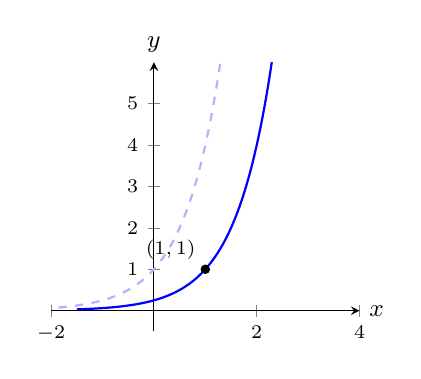
\begin{tikzpicture}
\begin{axis}[myaxis, xmin=-2,xmax=4,ymin=-0.5,ymax=6,
  ytick={1,2,3,4,5}]
\addplot[thick,blue,domain=-1.5:2.3]{4^(x-1)};
\addplot[thick,blue!30,dashed,domain=-2.5:1.3]{4^x};
\addplot[only marks,mark=*,mark size=1.5pt] coordinates {(1,1)};
\node[font=\scriptsize,above left] at (axis cs:1,1) {$(1,1)$};
\end{axis}
\end{tikzpicture}

(3) $y=\left(\dfrac{1}{4}\right)^{x}=4^{-x}$

$y=4^{x}$ の$y$軸対称．右下がり．

\begin{tikzpicture}
\begin{axis}[myaxis, xmin=-3,xmax=3,ymin=-0.5,ymax=6,
  ytick={1,2,3,4,5}]
\addplot[thick,blue,domain=-1.3:2.5]{4^(-x)};
\addplot[only marks,mark=*,mark size=1.5pt] coordinates {(0,1)};
\node[font=\scriptsize,above right] at (axis cs:0,1) {$(0,1)$};
\end{axis}
\end{tikzpicture}
}

\mondai{208}{グラフの対称移動の公式を用いて，次の関数のグラフをかけ．}
\kotae{
(1) $y=-4^{x}$：$y=4^{x}$ の$x$軸対称（$y\to-y$）

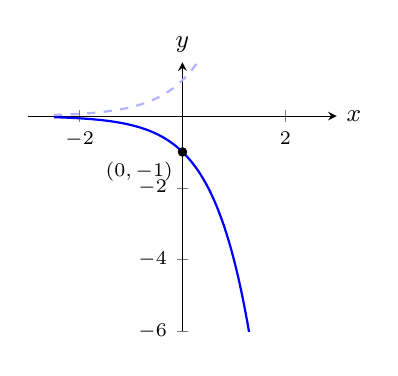
\begin{tikzpicture}
\begin{axis}[myaxis, xmin=-3,xmax=3,ymin=-6,ymax=1.5]
\addplot[thick,blue!30,dashed,domain=-2.5:1.3]{4^x};
\addplot[thick,blue,domain=-2.5:1.3]{-4^x};
\addplot[only marks,mark=*,mark size=1.5pt] coordinates {(0,-1)};
\node[font=\scriptsize,below left] at (axis cs:0,-1) {$(0,-1)$};
\end{axis}
\end{tikzpicture}

(2) $y=-4^{-x}$：$y=4^{x}$ の原点対称（$x\to-x$，$y\to-y$）

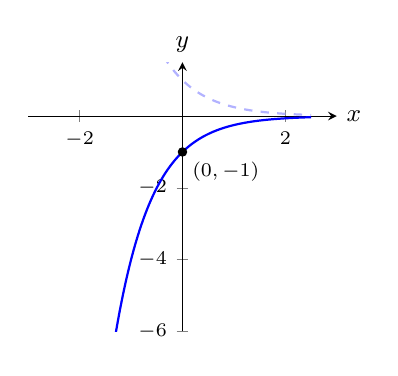
\begin{tikzpicture}
\begin{axis}[myaxis, xmin=-3,xmax=3,ymin=-6,ymax=1.5]
\addplot[thick,blue!30,dashed,domain=-1.3:2.5]{4^(-x)};
\addplot[thick,blue,domain=-1.3:2.5]{-4^(-x)};
\addplot[only marks,mark=*,mark size=1.5pt] coordinates {(0,-1)};
\node[font=\scriptsize,below right] at (axis cs:0,-1) {$(0,-1)$};
\end{axis}
\end{tikzpicture}
}

\mondai{209}{次の方程式を解け．}
\kotae{
指数方程式は，両辺の底をそろえて指数を比較する．

(1) $2^{2x}=2\sqrt[3]{2}=2^{1}\cdot2^{1/3}=2^{4/3}$

$2x=\dfrac{4}{3}$ → $x=\dfrac{2}{3}$

(2) $3^{-x+1}=\sqrt{243}=\sqrt{3^{5}}=3^{5/2}$

$-x+1=\dfrac{5}{2}$，$x=1-\dfrac{5}{2}=-\dfrac{3}{2}$

(3) $9^{x}-7\cdot3^{x}-18=0$

$3^{x}=t$ とおくと $t^{2}-7t-18=0$（$9^{x}=(3^{x})^{2}=t^{2}$）

$(t-9)(t+2)=0$．$t>0$ より $t=9$

$3^{x}=9=3^{2}$ → $x=2$
}

\mondai{210}{次の不等式を解け．}
\kotae{
底が1より大きい指数関数は単調増加なので，不等号の向きが保たれる．

(1) $8^{x}>16$

$(2^{3})^{x}>2^{4}$，$2^{3x}>2^{4}$

底 $2>1$ より $3x>4$ → $x>\dfrac{4}{3}$

(2) $\left(\dfrac{1}{5}\right)^{x+3}<\dfrac{1}{25}$

$5^{-(x+3)}<5^{-2}$

底 $5>1$ なので $-(x+3)<-2$，$-x-3<-2$，$-x<1$ → $x>-1$
}

\end{document}
